\documentclass[aspectratio=169,11pt]{beamer}
\usetheme{metropolis}
\usepackage[utf8]{inputenc}
\usepackage{graphicx}
\usepackage{booktabs}
\graphicspath{{../figures/}}

% ==== BEGIN RESULTS (injected from results.json) ====
\newcommand{\fLogReg}{0.26}
\newcommand{\fMLP}{0.40}
\newcommand{\accCNN}{0.70}
\newcommand{\fCNN}{0.68}
\newcommand{\accResnet}{0.80}
\newcommand{\fResnet}{0.78}
\newcommand{\bestlr}{3e{-4}}
\newcommand{\cnnparams}{1.44\,M}
\newcommand{\ablbase}{0.68}
\newcommand{\ablnoaug}{0.69}
\newcommand{\ablnobn}{0.72}
% ==== END RESULTS ====

\title{Classifying galaxy morphology with a CNN}
\subtitle{Galaxy10 DECaLS: baselines, a custom CNN, transfer learning, Grad-CAM}
\author{Philémon Vittet \and Patrick Yvan Eyike \and Sidi Hamadi \and
Abdelrahman Dahy \and Inès Lylia Zerdani}
\date{July 2026}

\begin{document}

\maketitle

\begin{frame}{The problem}
Galaxy Zoo asked \textbf{hundreds of thousands of volunteers} to sort galaxies by shape.
\begin{itemize}
  \item 17{,}736 color images, $256\times256$, from the DESI Legacy Imaging Surveys.
  \item 10 morphological classes: smooth, spiral (barred / tight / loose), edge-on, merging.
  \item \textbf{Can a CNN do that job automatically?}
\end{itemize}
\begin{center}
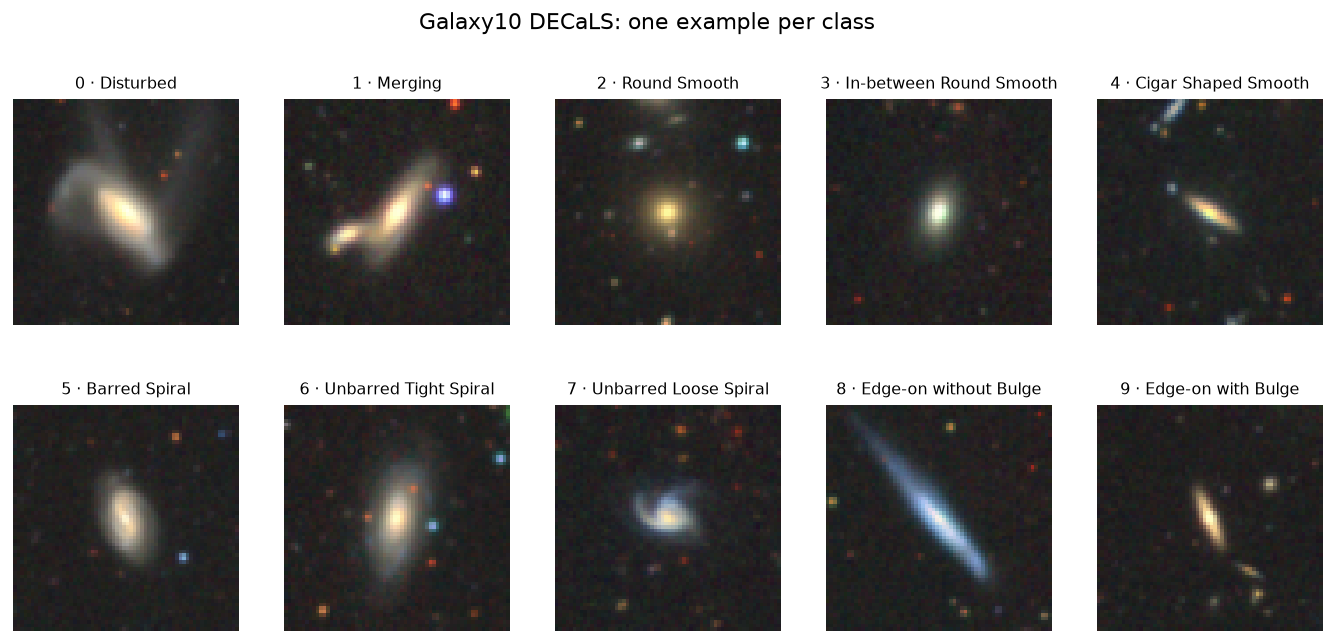
\includegraphics[width=0.82\textwidth]{samples.png}
\end{center}
\end{frame}

\begin{frame}{The data, and why it is hard}
\begin{columns}
\begin{column}{0.5\textwidth}
\begin{itemize}
  \item Strong class imbalance (factor $\sim$8): Cigar Shaped 334 vs Round Smooth 2{,}645.
  \item Neighboring classes look alike: tight vs loose spirals, round vs cigar.
  \item Noisy labels (volunteer votes).
  \item Official split: test set kept untouched; validation is 15\% of train.
\end{itemize}
\end{column}
\begin{column}{0.5\textwidth}
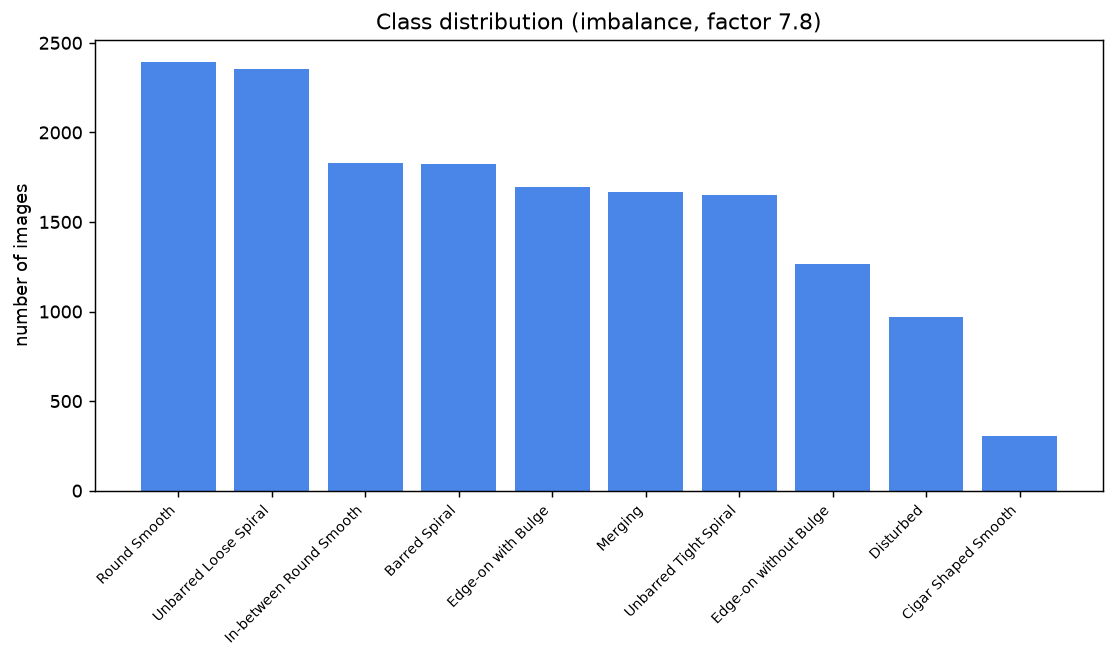
\includegraphics[width=\textwidth]{distribution.png}
\end{column}
\end{columns}
\end{frame}

\begin{frame}{Convolution in one slide}
A convolution slides the \textbf{same small filter} over the whole image:
\[ (I * K)_{i,j} = \sum_{m,n} I_{i+m,\,j+n}\,K_{m,n}. \]
\begin{itemize}
  \item \textbf{Weight sharing}: one filter everywhere $\Rightarrow$ few parameters, a motif detector.
  \item \textbf{Translation equivariance}: move the pattern, the response moves with it.
  \item This is a \textbf{symmetry built into the architecture}, exactly the spirit of symmetries
        in physics. A galaxy has no preferred orientation, so we also augment with rotations and flips.
\end{itemize}
\end{frame}

\begin{frame}{Our custom CNN}
\begin{columns}
\begin{column}{0.55\textwidth}
Four blocks \texttt{Conv 3x3 $\to$ BN $\to$ ReLU $\to$ MaxPool}, channels 32/64/128/256,
then adaptive pooling and a dense head.
\begin{itemize}
  \item Input $3\times64\times64$, halved at each pool.
  \item \textbf{\cnnparams{} parameters}, 73\% in the first dense layer.
  \item Weighted cross-entropy, Adam, cosine schedule, early stopping on macro-F1.
\end{itemize}
\end{column}
\begin{column}{0.45\textwidth}
\small
\begin{tabular}{ll}
\toprule
layer & output $(C,H,W)$ \\
\midrule
input & $3\times64\times64$ \\
block 1 & $32\times32\times32$ \\
block 2 & $64\times16\times16$ \\
block 3 & $128\times8\times8$ \\
block 4 & $256\times4\times4$ \\
head & $\to 10$ \\
\bottomrule
\end{tabular}
\end{column}
\end{columns}
\end{frame}

\begin{frame}{What does convolution buy us?}
\begin{columns}
\begin{column}{0.5\textwidth}
\begin{tabular}{lc}
\toprule
model & F1 macro \\
\midrule
Logistic regression & \fLogReg \\
MLP (pixels) & \fMLP \\
Custom CNN & \fCNN \\
ResNet18 (fine-tuned) & \fResnet \\
\bottomrule
\end{tabular}
\vspace{1em}

Baselines are blind to spatial structure. Convolution, then pretraining, explain the gain.
\end{column}
\begin{column}{0.5\textwidth}
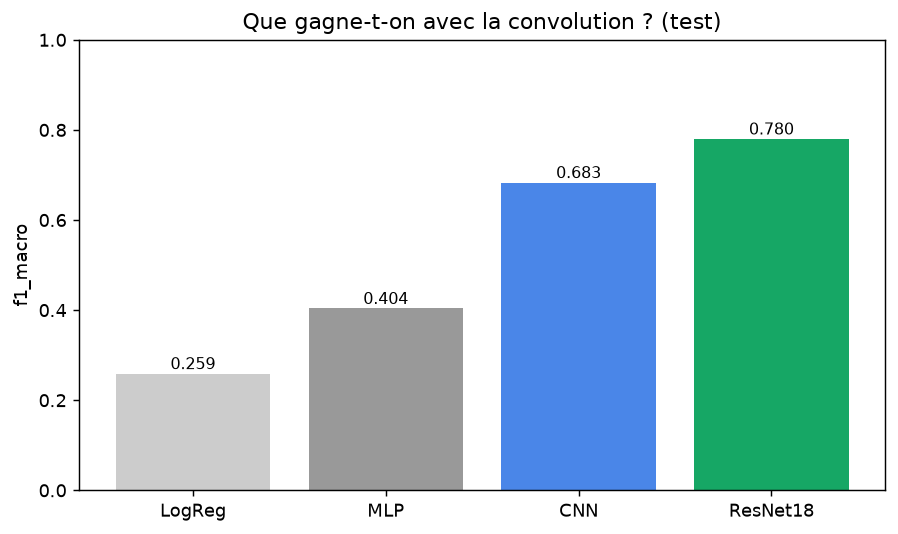
\includegraphics[width=\textwidth]{echelle.png}
\end{column}
\end{columns}
\end{frame}

\begin{frame}{Where it fails: confusion matrix}
\begin{center}
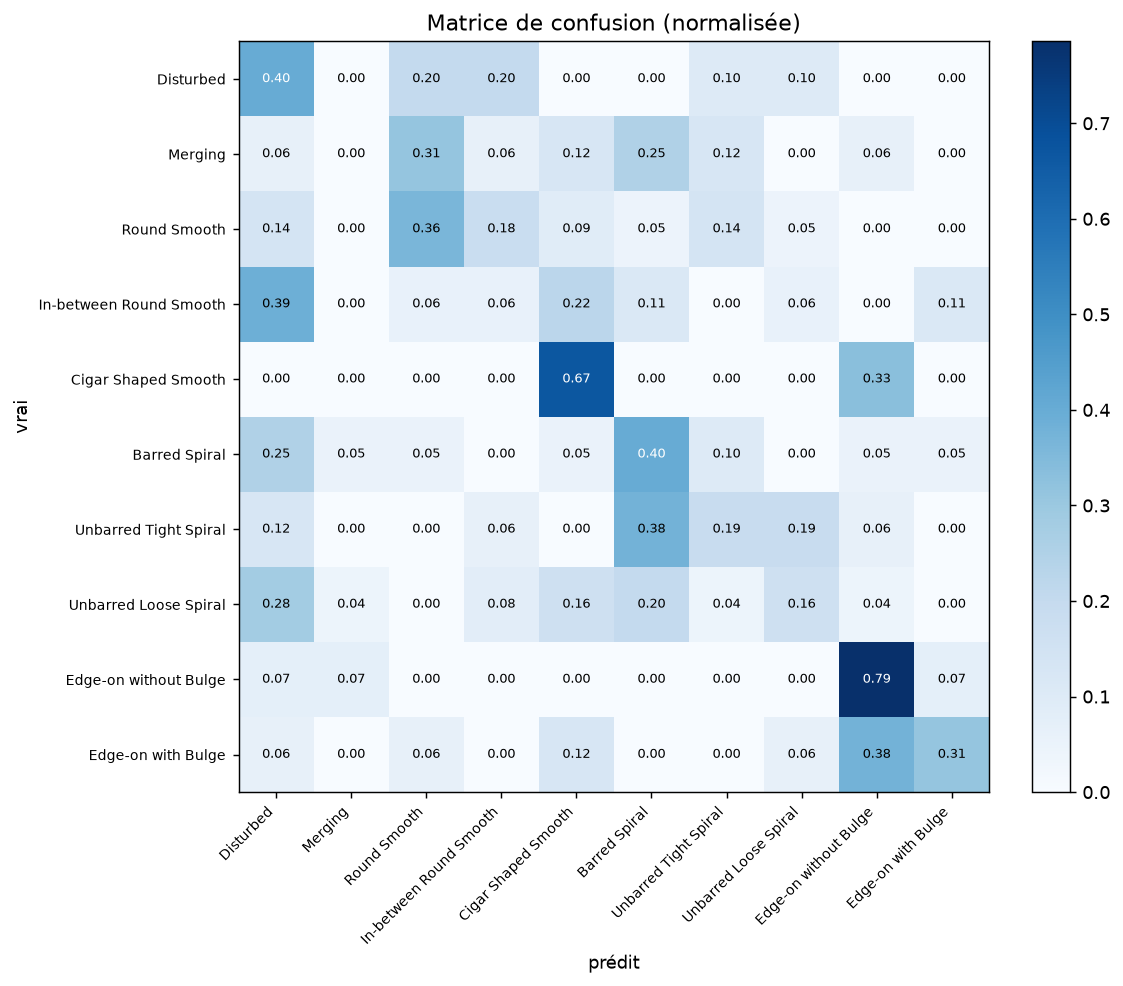
\includegraphics[width=0.6\textwidth]{confusion.png}
\end{center}
Errors concentrate between neighboring morphologies: loose vs tight spirals, and disturbed
galaxies spread across several classes. Disturbed (0.49 recall) and loose spirals (0.56) are
hardest; smooth and edge-on classes are near perfect.
\end{frame}

\begin{frame}{Grad-CAM: where the network looks}
\begin{center}
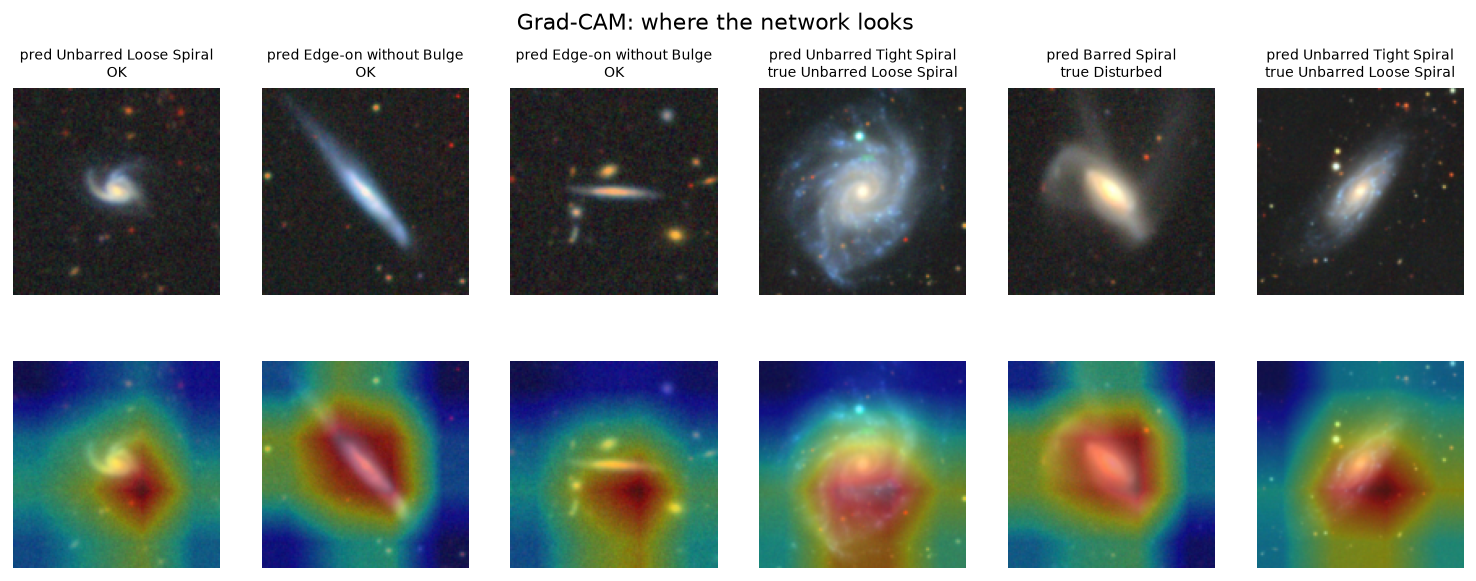
\includegraphics[width=0.96\textwidth]{gradcam_resnet.png}
\end{center}
On correct calls the heatmap sits on spiral arms, the bar, or the merging companion.
On errors it sometimes latches onto a neighbor or an artifact.
\end{frame}

\begin{frame}{Ablations and limits}
\begin{columns}
\begin{column}{0.5\textwidth}
\textbf{Ablations} (macro-F1, test):
\begin{itemize}
  \item full CNN: \ablbase
  \item no augmentation: \ablnoaug
  \item no BatchNorm: \ablnobn
\end{itemize}
Counterintuitive here: augmentation barely helps and removing BN even nudges F1 up. A
low-overfit, single-seed regime. BN still speeds convergence.
\end{column}
\begin{column}{0.5\textwidth}
\textbf{Limits}:
\begin{itemize}
  \item noisy Galaxy Zoo labels cap accuracy;
  \item class imbalance;
  \item training cost (64/128 px, partial tuning).
\end{itemize}
\end{column}
\end{columns}
\end{frame}

\begin{frame}{Conclusion}
\begin{itemize}
  \item A CNN reproduces Galaxy Zoo's morphological sorting: ResNet18 reaches
        accuracy \accResnet, macro-F1 \fResnet.
  \item The scale baseline $\to$ CNN $\to$ ResNet isolates the value of convolution.
  \item Grad-CAM shows the network uses real morphological structures.
  \item Key idea: convolution works on images because it \textbf{builds in a symmetry},
        translation equivariance, the way physics builds in symmetries.
\end{itemize}
\vspace{1em}
\centering \Large Thank you.
\end{frame}

\end{document}
